\documentclass[../thesis.tex]{subfiles}

\begin{document}


\section{Overview}
In this final chapter, we are motivated by the questions left unanswered by Chapter~\ref{chap:tmb_estimation}. In particular, previously we have relied on an established body of literature verifying the utility of \gls{tmb} as a proxy biomarker for response to immunotherapy. This has been advantageous in that is has allowed us not to concern ourselves with directly showing our derived mutation signatures are associated with improved response to immunotherapy (indeed, in many of the datasets exhibited in Chapter~\ref{chap:tmb_estimation} no such information was available), but rather just to predict \gls{tmb} as well as we can from \gls{wes} data. We need not worry whether \gls{tmb} is available as we can directly calculated it from \gls{tmb}. We now wish to interrogate further the direct relationship between genomic signatures (such as \gls{tmb}) derived from targeted gene panel sequencing and .


\section{Survival analysis \label{sec:survival}}


\subsection{Survival times}

Survival analysis concerns modelling the amount of time elapsing before a given event occurs. In medical settings, this is often time-to-death analysis, but the same framework is used to approach other events, both medical (e.g. relapse or visit to hospital) and non-medical (machine lifetime, customer churn, etc.). We will refer here to the generic `event' as death (since this is our main application case), generic `samples' as patients, and time-to-event measures as survival times. For a patient $i$, we will typically refer to survival times with either a lower case $t_i$ (for observations) or upper case $T_i$ (for random variables). We note the following properties we might expect from survival times, both of which influence decisions around modelling:
\begin{enumerate}
    \item `Survival times are continuous' ($t_i \in \mathbb{R}$). This is intuitively true in many situations, but we often only have access to discrete bins (e.g. months). This can lead to modelling complexities such as the presence of exact ties between observations.
    \item `Survival times are positive' ($t_i > 0$). This introduces another important notion: that survival times are \emph{relative} to some other point in time. The definition of this point in time can be important and varied between (and sometimes within) studies.
\end{enumerate}
Point two above emphasises the importance of appropriate definition of starting time for interpreting survival times. Of perhaps even greater subtlety can be the definition of end time. In the cases we're addressing, this tends to be patient death (often referred to as \gls{os}). However, we are often implicitly interested in analysing the likelihood of dying from one particular factor (e.g. lung cancer). In many studies, death from other causes (which, complexifying matters further, may be related non-trivially to the factor under study, e.g. dying from cardiac arrest while suffering lung failure) is counted identically to death from the cause of interest. In others, patients who die for other reasons may be excluded from the study. Both approaches have issues, but the latter case is an example of a more ubiqituous phenomenon in survival studies (at least those pertaining to human patients): \emph{censoring}.

\subsection{Censoring}
In the previous section, we discussed a particular (in fact, quite complex and nuanced), form of censoring, but other forms are more clear cut. Censoring in general refers to any consideration that means that we do not get to observe the patient until they die of the cause of interest. We therefore might think of the example above as `censoring by death from other cause'. Here are two further types of censoring:

\begin{enumerate}
    \item `Censoring by continued survival'. This form of censoring is universal to human survival studies. In short: we cannot wait for everyone in a study to die, and we certainly can't force them to! At some point the study ends, and some participants may remain alive. We know (or suspect) that given enough time they would eventually die from the cause of interest, but all we know is that they survived at least as long as they had survived at the end of the study.
    \item `Censoring by terminated participation'. This, broadly speaking, covers everything else. There are a variety of reasons patients may have to be removed from the cohort under observation during the progress of a study. These include medical non-compliance (e.g. refusing to take the treatment assigned to them), loss of follow-up (e.g. not responding to monthly requests for information), or reassignment due to some other protocol (e.g. being switched arms on a clinical trial for ethical reasons if it appears another treatment is clearly more beneficial).
\end{enumerate}

To address censoring, we use the following notation. For a patient $i$, we let $c_i \in \mathbb{R}^{+}$ (or $C_i$ for a random variable) denote the time at which the patient is removed from further observation. We therefore observe only the following: $y_i \in \mathbb{R}^{+}$ (or $Y_i$ for random variable) is the time of final follow-up, i.e. $y_i = \min(c_i, t_i)$; and $\delta_i$ (or $\Delta_i$) for censorship status, i.e. $\delta_i = \mathbbm{1}\{t_i \leq c_i\}$. 

The core question for statistical modelling of survival is, therefore, how to make inferences about the behaviour of the random variables $T_i$ from observation only of a given set of $n$ pairs $\{(y_i, \delta_i)\}_{i=1}^{n}$. In general we assume these tuples of observations (and potential future observations) to be realisations of independent and identically distributed random variables, and so refer to this underlying joint distribution without reference to sample $i$, i.e. we consider ($T, C, \Delta)$.  We discuss in the next section some common practices for performing inference on these targets.
   
\subsection{Modelling approaches}
We've now defined and introduced notation for the targets of inference in a survival modelling setting. In this section we'll describe some common approaches for performing this modelling, and in particular for modelling survival conditional on a further random vector of features $X$. 

We begin by defining \textit{hazard}. While it is possible to characterise the distribution of survival times $T$ in a variety of ways, hazard is common as it is both interpretable and easy to work with. For the distribution $T$, we define hazard $h(t)$ as a function of time $t$ as the instantaneous rate of death at time $t$, given survival up until time $t$, via:
\[
    h(t) := \lim_{\delta t \rightarrow 0} \frac{\mathbb{P}(T \in [t, t + \delta t] | T > t)}{\delta t}.
\]
We also define the \textit{survival} function $S(t)$ as $\mathbb{P}(T > t)$. We may then observe that hazard is expressible as 
\begin{align*}
    h(t) & = \lim_{\delta t \rightarrow 0} \frac{\mathbb{P}(T > t) - \mathbb{P}(T > t + \delta t)}{\mathbb{P}(T > t) \delta t} \\
    & = \frac{1}{S(t)} \lim_{\delta \rightarrow 0} \frac{S(t) - S(t + \delta t)}{\delta t}\\
    & = - \frac{1}{S(t)} \frac{d}{dt} S(t)\\
    & = - \frac{d}{dt} \log S(t). 
\end{align*}
Finally note that $\frac{dS}{dt} = - f(t)$, where $f(t)$ is the probability density function for $T$, so we may also write $h(t) = \frac{f(t)}{S(t)}$. This is consistent with the intuition that hazard denotes rate of death, scaled by likelihood of survival so far. Often when fitting predictive models, we use hazard as the target of prediction given inputs $x$, aiming to estimate $h(t|x)$. Before we move on to this case, however, we'll discuss a few more properties of hazard. It can be useful to define the cumulative hazard function $H(t) = \int_{0}^{t}h(u)du$. We can then write down further useful relations between hazard, cumulative hazard, and density. Firstly note that 
\begin{align*}
H(t) & := \int_{0}^{t}h(u)du \\
& = -\int_{0}^{t}\frac{d}{du} \big(\log S(u)\big) du  \\
& = - \big[\log S(u) \big]_{0}^{t} \\
& = -\log S(t),
\end{align*}
so we can also express $H(t)$ in terms of the survival function. Likewise we can express $f(t)$ simply in terms of hazard via
\[ f(t) = h(t)S(t) = h(t)\exp (-H(t)).\]
From this last relationship we can quickly see that under an assumption of \emph{constant hazard} $h(t)=\lambda$, survival times will follow an exponential distribution, with density function $f(t) = \lambda \exp(-\lambda t)$, with mean $\lambda^{-1}$ and variance $\lambda^{-2}$.

However, as mentioned above, a single model for all survival times is not sufficient for most purposes. In general we want to learn about the effect of some covariates on survival time. We therefore introduce a random (potentially vector-valued) variable $X$ taking values in $\mathbb{R}^p$, and define the following conditional versions of survival and hazard functions:
\begin{align*}
    h(t|x) & := \lim_{\delta t \rightarrow 0} \frac{\mathbb{P}(T \in [t, t + \delta t] | T > t, X = x)}{\delta t} \\
    S(t|x) & := \mathbb{P}(T > t | X = x).
\end{align*}
Note that the same relationships as above hold. When making decisions around modelling, assumptions about the behaviour of these two functions are typically the starting point. We'll here evaluate two common assumptions, based on restricting the functional form of each of these two functions respectively.

\subsubsection{The proportional hazards assumption}
Proportional hazards models are based on the assumption that changes in a given covariate have the effect of increasing hazard by a constant factor across all time points. We state this formally as follows: that there exist functions $h_0: \mathbb{R}^+ \rightarrow \mathbb{R}^+$ and $\theta: \mathbb{R}^p \rightarrow \mathbb{R}^+$ such that 
\[h(t|x) = h_0(t) \theta(x). \]
In practice the function $\theta$ is often chosen to be $\theta(x) = \exp (- \beta^T x)$ for parameter $\beta \in \mathbb{R}^p$ to be fitted. In this case $h_0(t)$ is left to be fitted flexibly (although this is not necessary for inferring $\beta$, making the resulting model (the Cox model; \citealp{cox_regression_1972}) semi-parameteric. Note that we can derive the resultant form of the survival function as $S(t|x) = S_0(t)^{\theta(x)}$, where $S_0(t) = \exp(-\int_{0}^{t}h_0(u)du)$.


\subsubsection{The accelerated failure time assumption}
Accelerated failure time models \citep{wei_accelerated_1992} are based on the assumption that changes in a given covariate have the effect of scaling the entire lifetime of a patient by a constant factor. This is formalised by position that there exist functions $S_0: \mathbb{R}^+ \rightarrow [0,1]$ and $\theta: \mathbb{R}^p \rightarrow \mathbb{R}^+$ such that 
\[S(t|x) = S_0(\theta(x)t).\]
As for proportional hazards, the function $\theta$ is often chosen to be $\theta(x) = \exp (-\beta^T x)$. Again as above, we may use this restriction to infer the form of the hazard function as $\theta(x)h_0(\theta(x)t)$, where $h_0(t) = -\frac{d}{dt} \log S_0(t)$. The function $S_0(t)$ is often chosen to be the exponential survival function $e^{-t}$.

Note that the proportional hazards and accelerated failure time assumptions are not mutually exclusive. Consider for example the following setting: $T$ is Weibull distributed with parameters $\lambda, k$, i.e. has cumulative distribution function $1- \exp((t/\lambda)^k$. Now suppose that the parameter $\lambda$ is given by $\lambda = \lambda_0 \exp(\beta^T x)$. We then have that 
\[S(t|x) = \exp\big(-t^k\lambda_0^{-k}\exp( -\beta^Tx)\big), \]
which satisfies the correct form for the accelerated failure time assumption with $S_0(t) = \exp(-t^k)$ and $\theta(x) = \lambda_0^{-k}\exp(\beta^Tx)$. We can also show that the hazard is given by 
\[h(t|x) = kt^{k-1}\lambda_0^{-k} \exp(-k\beta^Tx), \]
satisfying the proportional hazards assumption with $h_0(t) = k\lambda_0^{-k}t^{k-1}$ and $\theta(x) = \exp(-k\beta^Tx)$. 

\subsection{Fitting survival models}

\section{Heterogeneous treatment effect}
\Glspl{hte} refer to interactions between the effect of some intervention, or \emph{treatment}, and some other covariates. In particular we aim to predict, from some input covariates, the change in outcome for a given sample upon applying a given intervention, while by definition never being able to observe a sample when the given treatment has both been applied and not been applied (referred to as the \emph{fundamental problem for causal inference}; \citealp{holland_statistics_1986}). Similar to how we approached survival, we first establish some terminology for causal inference without considering prediction based on covariates, and then move on to consider \glspl{hte}.

\subsection{Potential outcomes}
We first consider the following scenario: a response variable $Y$ taking values in $\mathcal{Y}$, a binary treatment indicator variable $A$ taking values in $\{0,1\}$, and a variable of covariates (also sometimes referred to as \emph{confounders}) $X$ taking values in $\mathcal{X} \in \mathbb{R}^p$. We want to gauge the effect of altering the treatment $A$ on the outcome $Y$. A natural quantity to estimate might be
\[\bbE[Y | A = 1] - \bbE[Y | A = 0].\]
However, if both $Y$ and $A$ depend on $X$, we might observe some spurious dependencies. We therefore want to develop a framework in which we are comparing reasonable \emph{potential outcomes} of $Y$ in a hypothetical alternate universe in which we had intervened/not intervened to change $A$.

Further to the above, we propose the following. Let $Y^{(0)}, Y^{(1)}$ refer to potential outcomes taken by $Y$ under intervention with $A=0,1$
respectively. We may therefore say that $Y=Y^{(A)}$. In the alternate notation of do-calculus \citep{pearl_causal_1995, pearl_-calculus_2012}, we would say that $\mathbb{P}(Y^{(a)} = y) := \mathbb{P}(Y = y |  \text{do}(A=a))$. We make two further assumptions: 
\begin{enumerate}
    \item The propensity function has global support over the support of $X$, i.e. 
    \[\pi(x) := \mathbb{P}(A=1 | X = x) \  \text{is such that} \ \pi(X) \in (0,1) \ \text{almost surely.}\]
    \item Treatment is essentially random given $X$, i.e.
    \[\{Y^{(0)}, Y^{(1)}\} \perp\!\!\!\perp A | X. \]
\end{enumerate}
These are considered sufficient to estimate the \emph{\gls{ate}}, defined as $ATE := \bbE[Y^{(1)} -Y^{(0)}]$ to be identifiable, since 
\begin{align*}
    ATE & = \bbE[Y^{(1)} - Y^{(0)} ] & \\
    & = \bbE[\bbE[Y^{(1)} - Y^{(0)} | X]] & \text{(by the tower property)} \\
    & = \bbE[\bbE[Y^{(1)} | X]] - \bbE[\bbE[Y^{(0)} | X]] & \\ 
    & = \bbE[\bbE[Y^{(1)} | X, A = 1]] - \bbE[\bbE[Y^{(0)} | X, A = 0]] & \text{(by Assumption~2)} \\
    & = \bbE[\bbE[Y | X, A = 1] - \bbE[Y | X, A = 0]], & \label{eq:ate}
\end{align*}
and $X$, $Y$ and $A$ are all observed quantities. Assumption~1 establishes that we can expect to observe samples with both $A=0$ and $A=1$ across the support of $X$. Methods for estimation of $ATE$ have been proposed for a variety of modelling assumptions and contexts \citep{reiersol_confluence_1945, thistlethwaite_regression-discontinuity_1960, rosenbaum_central_1983, abadie_semiparametric_2005, craig_natural_2017, roth_whats_2023}. One common such method is propensity score matching, which relies on partitioning observations into groups with approximately equal propensity scores. Note that 
\begin{align*}
    \mathbb{P}(A=1 | \pi(X), Y^{(1)}, Y^{(0)}) & = \bbE[A | \pi(X), Y^{(1)}, Y^{(0)}] & \\
    & = \bbE[\bbE[A | X, Y^{(1)}, Y^{(0)}] | \pi(X), Y^{(1)}, Y^{(0)}] & \text{(by the tower property)}\\
    & = \bbE[\bbE[A|X]|\pi(X), Y^{(1)}, Y^{(0)}] & \text{(by Assumption~2)} \\
    & = \bbE[\pi(X) | \pi(X), Y^{(1)}, Y^{(0)}] & \text{(by definition of propensity)} \\
    & = \pi(X) = \mathbb{P}(A=1|\pi(X)), &
\end{align*}
so that $\{Y^{(0)}, Y^{(1)}\} \perp\!\!\!\perp A | X \Rightarrow \{Y^{(0)}, Y^{(1)}\} \perp\!\!\!\perp A | \pi(X)$ (this is due to \citealt{rosenbaum_central_1983}). We can then say that
\[ATE = \bbE[\bbE[Y|\pi(X), A=1] - \bbE[Y|\pi(X), A=0]].\]
To estimate the \gls{ate} we therefore need only to average over the marginal distribution of $\pi(X)$ rather than the entire marginal distribution of $X$, which can be particularly useful when $X$ is high-dimensional.

While it is often useful to gauge the utility of a treatment across an entire population via the ATE, it does not necessarily make any progress towards recommending whether treatment will benefit a given patient. For this, we need heterogeneous, conditional, or individual treatment effect, discussed in the following section.

\subsection{Treatment with inputs}
We now define \glspl{hte} (also referred to as 
\glsxtrlong{cate}), which will be our tool to make predictions at the individual level. We define the treatment function $\tau: \mathcal{X} \rightarrow \mathcal{Y}$ as follows:
\begin{align*}
    \tau(x) & := \bbE[Y^{(1)} | X =x] - \bbE[Y^{(0)} | X=x] \\
    & = \mu_1(x) - \mu_0(x) 
\end{align*}
where $\mu_a(x) := \bbE[Y^{(a)}|X=x]$ is the conditional regression function for potential outcome $A=a$. Note that the logic demonstrated in the derivation of the identifiability of the \gls{ate} applies to conditional treamtent effect and we can also say that (under Assumptions~1~and~2) we have that $\mu_a(x) = \bbE[Y|X=x,A=a]$. This means that one viable strategy for estimation of \glspl{hte} is simply to estimate $\mu_0,\mu_1$ with $\muhat_0, \muhat_1$ respectively, and $\tau$ with $\hat{\tau}(x) := \muhat_1(x) - \muhat_0(x)$. We will discuss this strategy, known as a $T$-Learner, and its potential shortcomings in the next section.

While we've introduced \glspl{hte} in order to be able to make decisions at the individual level, it is worth pointing out that it is in general distinct from individual treatment effect \citep{vegetabile_distinction_2021}. In essence, since heterogeneous effect only requires conditioning on some set of covariates satisfying the strong ignorability assumption, it need not contain all relevant information about $Y$. In particular, suppose we are given a variable $X$ satisfying strong ignorability. Then we can form $X'=(X,Z)$ for any other covariate $Z$ estimate an identifiable \glspl{hte}. To emphasise the difference between truly individual treatment effects and those based merely on conditioning on some strongly ignorable set of variables, some authors use the term \emph{\gls{cate}} \citep{vegetabile_distinction_2021}.

\subsection{Meta-learner strategies}
\label{sec:metalearners}
As mentioned in the above, we divide strategies for estimating \glspl{hte} into general classes of \emph{meta-learner} \citep{kunzel_metalearners_2019, curth_nonparametric_2021}. Each of these relies on some baseline strategy for fitting a regression function, and applies it to some combination of target functions. We describe a few below.

\begin{enumerate}
    \item \label{tech:tlearner} $T$-Learners: this base strategy centred on the identifiability of the conditional regression functions $\mu_0, \mu_1$. We simply split our dataset into two portions such that, according to observed values, the treatment variable takes the values $A=0$ or $A=1$. We then fit $\muhat_0(x), \muhat_1(x)$ separately on these two subsets, and define:
    \[ \hat{\tau}(x) := \muhat_1(x) - \muhat_0(x).\]
    \item $S$-Learners: a small variation on $T$-Learners, indeed in some simple cases identical. With this approach we jointly fit $\muhat(x,a)$ such that $\muhat(x,0) \approx \mu_0(x)$ and that $\muhat(x, 1) \approx \mu_1(x)$, then define:
    \[\hat{\tau}(x) := \muhat(x,1) - \muhat(x,0).\]
    \item \label{tech:ipw} Methods based on \emph{pseudo-outcomes} define some intermediate statistic that can be estimated based on observed data. The simplest is based on the Horvitz-Thompson transformation \citep{horvitz_generalization_1952}, also known as \gls{ipw}. We define:
    \[\Tilde{Y}_{IPW} := \Big(\frac{A}{\pihat(X)} - \frac{1-A}{1-\pihat(X)}\Big)Y, \]
    relying on the observation that, if $\pihat(x) = \pi(x)$, then $\bbE[\Tilde{Y}_{IPW} | X =x] = \tau(x)$. The advantage of this approach is that the quantity $\Tilde{Y}_{IPW}$ only depends on observable quantities, and so can be estimated from the full dataset.
    \item Hybrid methods comprise some combination of strategies based on fitting potential regression functions (for example via $T$-Learners) and pseudo-outcomes. These include $X$-Learners as proposed by \citet{kunzel_metalearners_2019} -- for which special cases have been investigated further by \citet{curth_nonparametric_2021} -- and generalised `doubly robust' estimators proposed by \citet{kennedy_optimal_2020}. In this context, double robustness refers to a learner that produces consistent estimates even if only one of $\muhat$ and $\pihat$ are correctly specified.
    \item \citet{shalit_estimating_2017} proposed a method based on distributional regularisation such that, by construction, information is shared between estimated regression functions $\muhat_0$ and $\muhat_1$. This level of information sharing is tunable via a regularisation parameter that may itself be selected by cross-validation (more on this later).
\end{enumerate}

\subsection{Double robustness} \label{sec:doublerobustness}
In settings in which the \gls{cate} demonstrates complex structure, it is an important and open challenge to provide estimators that are demonstrably robust and flexible. This ideally includes robustness in cases of various forms of model misspecification. To heuristically motivate these cases, we next consider two example settings. As well as motivating the discussion of double robustness that is to come, they also serve to develop our intuition as to when some of the strategies described in Section~\ref{sec:metalearners}, in particular $T$-Learners and estimators based on \gls{ipw}. They are as follows.

\begin{example}{\textbf{(Simulation Setting 1)}} \label{ex:ipw_better}
We model observations of the triple $(X, A, Y)$, with $X$ and $Y$ taking values in $\mathbb{R}$ and $A$ taking values in $\{0,1\}$, as independent triplet realisations of the joint distribution described as follows:

\begin{align*}
X & \sim \mathrm{Norm}(0, 1) \\    
A \ | \ (X = x) & \sim \mathrm{Bern}\Big(\frac{1}{1 + \exp(-x)}\Big) \\ 
Y \ | \ (X = x) & \sim \begin{cases}
      x^2 + x & \text{where} \ A = 1\\
      x^2 & \text{where} \ A = 0
    \end{cases}
\end{align*}
\end{example}

Example~\ref{ex:ipw_better} aims to model a setting in which estimation of the individual conditional regression functions $\mu_a(x)$ is difficult, but estimation of both the propensity function $\pi(x)$ and the \gls{cate} $\tau(x)$ is simple. Note that here the functions $\mu_a(x)$ are not intrinsically complex (we could easily fit them with polynomial regression), but we will attempt to model them with linear regression models than cannot adequately capture them. This is therefore a case of model misspecification rather than one of functional complexity, but we will demonstrate the same points. \citet{kennedy_towards_2022} gives similar examples in which more general nonparametric models are used and the issue is genuinely one of functional complexity without model misspecification, but the underlying phenomena and results are the same.


\begin{example}{\textbf{(Simulation Setting 2)}} \label{ex:t_better}
We model observations of the triple $(X, A, Y)$, with $X$ and $Y$ taking values in $\mathbb{R}$ and $A$ taking values in $\{0,1\}$, as independent triplet realisations of the joint distribution described as follows:

\begin{align*}
X  & \sim \mathrm{Norm}(0, 1) \\    
A \ | \ (X = x) & \sim \mathrm{Bern}\Big(\frac{1}{1 + \exp(-\cos(2x))}\Big) \\ 
Y \ | \ (X = x) & \sim \begin{cases}
      3x/4 & \text{where} \ A = 1\\
      -x/4 & \text{where} \ A = 0
    \end{cases}
\end{align*}
\end{example}

Example~\ref{ex:t_better}, by constrast with Example~\ref{ex:ipw_better}, aims to model a setting in which estimation of the propensity function $\pi(x)$ is difficult, but estimation of the conditional regression functions $\mu_a(x)$ is easy. 

Almost by construction, these example settings are such that for Example~\ref{ex:ipw_better} the \gls{ipw} estimator defined in \eqref{tech:ipw} will outperform the $T$-Learner \eqref{tech:tlearner}, and vice versa for Example~\ref{ex:t_better}. We find that this does indeed bear out in Figure~\ref{fig:comp_t_ipw}. Here we have generated 100 samples from each of the models specified, applied each of the $T$-Learner and \gls{ipw} strategies with linear regression models providing each of the estimation procedures (and logistic regression applied to produce an estimated propensity function $\pihat(x)$), and applied the resultant estimated \gls{cate} function to each of the training set data points. The true \gls{cate} function (in each case $\tau(x) = x$) is given for comparison. We do indeed see that our expectations are borne out in each of these settings, with the \gls{ipw} method performing very well on Simulation Setting~1 and the $T$-Learner performing very well on Simulation Setting~2.

These illustrative cases are representative of two potential sources of error via model misspecification. The aim of double robustness is to create estimators of \gls{cate} that work in each of the regimes we've illustrated. Formally, we aim to produce consistent estimates even if one of $\pi(x)$ or $\mu_a(x)$ are misspecified. Practically, this tends to work via weighted combinations of \gls{ipw} and $T$-Learner estimates. \citet{kennedy_towards_2022}, building upon work from \citet{nie_quasi-oracle_2021} and others, define the DR-Learner as follows (again depending upon an arbitrary regression function). 

\begin{technique}{(\textbf{DR-Learner})}
Given fitting methods for estimating propensity scores and conditional regression outcomes, the DR-Learner consists of two steps (\citet{kennedy_towards_2022} define an optional third to incorporate sample splitting and cross-validation, but for simplicity we omit this here).
\begin{enumerate}
    \item Nuisance function training:
    \begin{itemize}
        \item Construct estimates $\pihat$ of the propensity scores $\pi$.
        \item Construct estimates $(\hat{\mu_0}, \hat{\mu_1})$ of the regression functions $(\mu_0, \mu_1)$.
    \end{itemize}
    \item Pseudo-outcome regression: construct the pseudo-outcome
    \[\Tilde{Y}_{DR} := \frac{A - \pihat(X)}{\pihat(X)(1-\pihat(X))}\Big( Y - \muhat_A(X)\Big) + \muhat_1(X) - \muhat_0(X),\]
    and regress it on covariates X, yielding
    \[\hat{\tau}_{DR}(x) = \hat{\bbE}[\Tilde{Y}_{DR} | X = x],\]
    where the symbol $\hat{\bbE}$ denotes estimated expectation under the chosen regression function.
\end{enumerate}
\end{technique}

\begin{figure}[!tpb] 
\centering
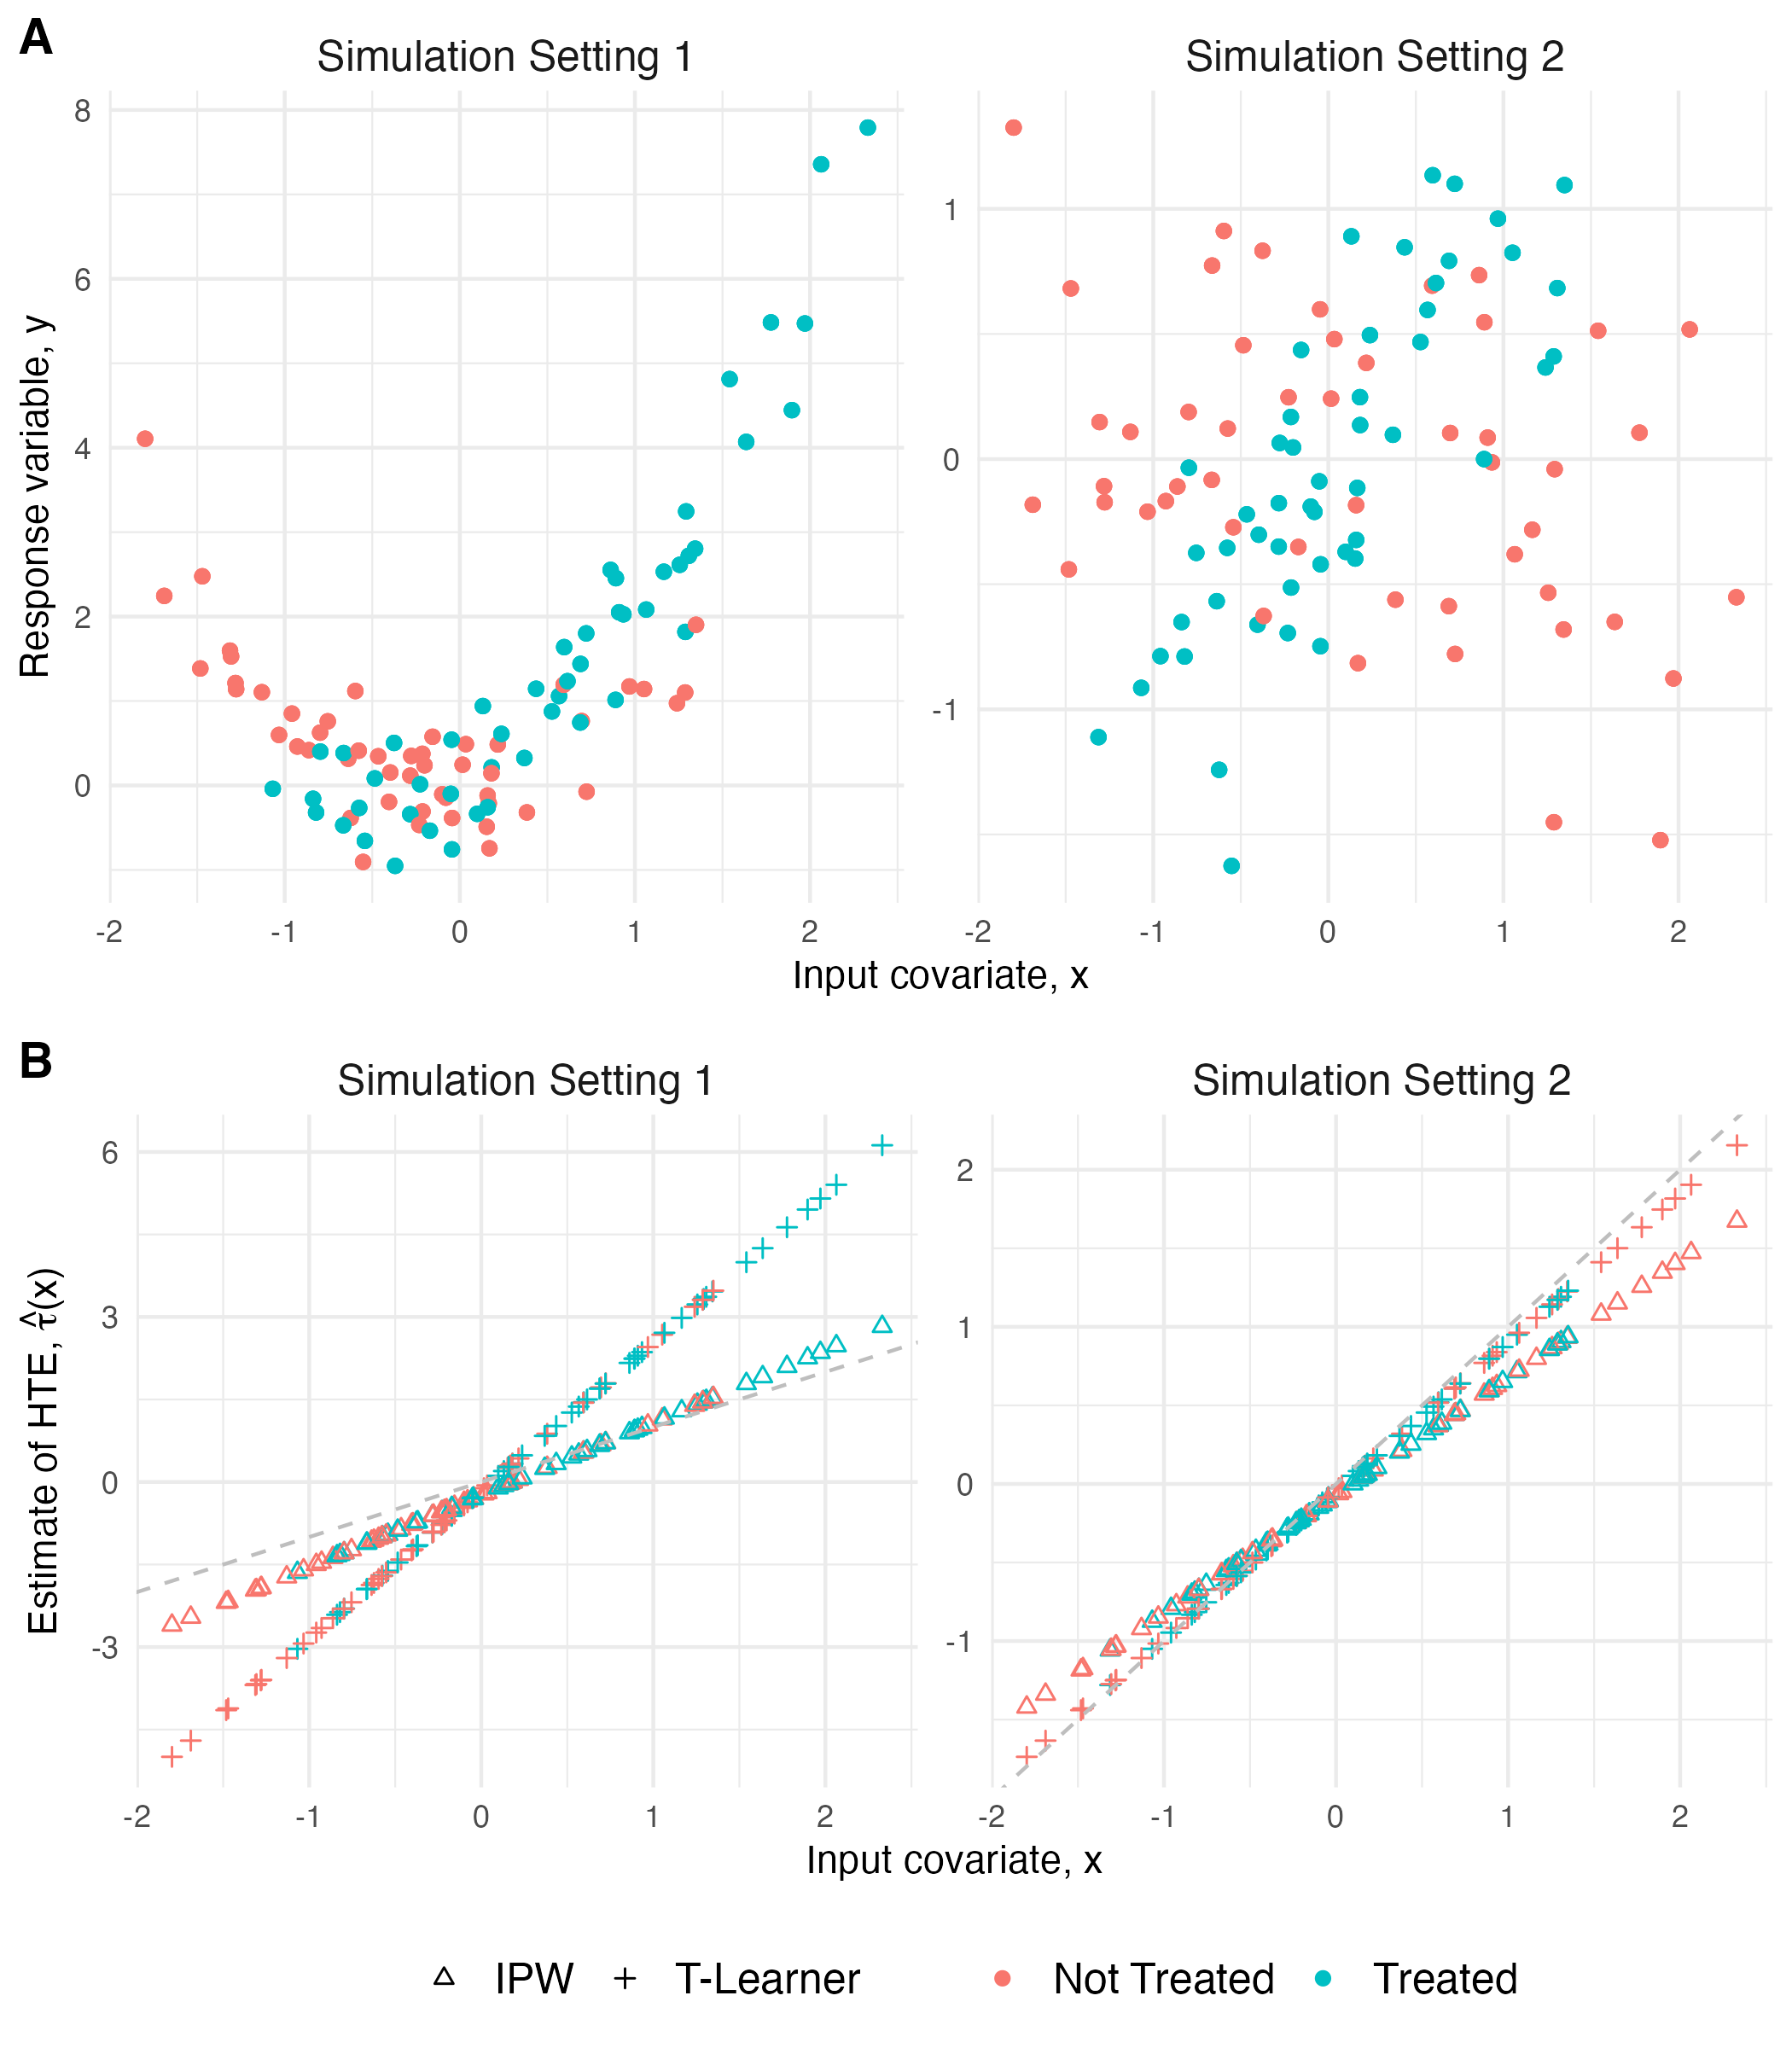
\includegraphics[width=\textwidth]{figures/chapter4/comp_figure_without_dr.png}
\caption{Simulation Settings~1~and~2 with \textbf{A}: the response variable $y$, and \textbf{B}: estimates of $\hat{\tau}(x)$ for each simulated data point according to the $T$-Learner (cross) and \gls{ipw} (triangle) strategies. The true \gls{cate}, $\tau(x)$, is shown with a grey dashed line.  \label{fig:comp_t_ipw}}
\end{figure}
Under certain conditions on stability, the DR-Learner can be shown to produce optimal convergence rates amongst classes of models based on composition of \gls{ipw} and conditional regression functions. We won't go into these conditions in detail here, but can begin to appreciate the underlying ideas by investigating the two extreme cases we've discussed. Firstly, let's assume in Step~(1) of the DR-Learner, we correctly estimate propensity (i.e. $\pihat = \pi$) but do not correctly estimate our conditional regression functions (i.e. $(\muhat_0, \muhat_1) \neq (\mu_0, \mu_1)$). We can then write that 
\begin{align*}
    \Tilde{Y}_{DR} & =  \frac{A - {\pi}(X)}{{\pi}(X)(1-{\pi}(X))}\Big( Y - \muhat_A(X)\Big) + \muhat_1(X) - \muhat_0(X) \\
    & = \frac{A - {\pi}(X)}{{\pi}(X)(1-{\pi}(X))}\Big(A\big(Y^{(1)} - \muhat_1(X)\big) + (1-A)\big(Y^{(0)} - \muhat_0(X) \big)\Big) \\
    & \hspace{50pt} + \muhat_1(X) - \muhat_0(X)
\end{align*}
and therefore that
\begin{align*}
    \bbE[\Tilde{Y}_{DR} | X=x]  & = \frac{1}{\pi(x)(1-\pi(x))} \Big(\bbE[AY^{(1)} - A\muhat_1(x) - A\pi(x)Y^{(1)} + A\pi(x)\muhat_1(x) \ - \\
    & \hspace{50pt} (1-A)\pi(x)Y^{(0)} + (1-A)\pi(x)\muhat_0(x) \ | \ X=x ] \Big) + \muhat_1(x) - \muhat_0(x) \\ 
    & = \frac{1}{\pi(x)(1-\pi(x))} \Big( \pi(x)\mu_1(x) - \pi(x)\muhat_1(x) - \pi(x)^2\mu_1(x) + \\
    & \hspace{50pt} \pi(x)^2\muhat_1(x) - (1-\pi(x))\pi(x)\mu_0(x) + (1-\pi(x))\pi(x) \muhat_0(x) \Big) + \\
    & \hspace{50pt} \muhat_1(x) - \muhat_0(x) \\
    & = \frac{1}{\pi(x)(1-\pi(x))]} \Big( \pi(x)\big(\mu_1(x) - \muhat_1(x) - \pi(x)(\mu_1(x) - \muhat_1(x)) \big) - \\
    & \hspace{50pt} \pi(x)(1-\pi(x))\big( \mu_0(x) - \muhat_0(x) \big) \Big) + \muhat_1(x) - \muhat_0(x) \\
    & = (\mu_1(x) - \muhat_1(x)) - (\mu_0(x) - \muhat_0(x)) + \muhat_1(x) - \muhat_0(x) \\ 
    &= \mu_1(x) - \mu_0(x) = \tau(x),
\end{align*}
where here in the first equality we are leveraging that $A^2 = A$ and (equivalently) that $A(1-A) = 0$, and in the second equality we make use of the fact that $Y\perp A \ | \ X$ and that $\mu_a(x) := \bbE[Y^{(a)}|X=x]$.

Secondly, let's now assume we've estimated the conditional regression functions well (so that $(\muhat_1, \muhat_0) = (\mu_1, \mu_0)$). Then we can say that 

\begin{align*}
    \bbE[\Tilde{Y}_{DR} | X = x] & = \bbE [\frac{A - \pihat(x)}{\pihat(x)(1 - \pihat(x)} \Big( A (Y^{(1)} - \mu_1(x)) + \\
    &\hspace{50pt} (1-A)(Y^{(0)} - \mu_0(x)) \Big) \ | \ X=x] \ +  \mu_1(x) - \mu_0(x)  \\
    & = \frac{1}{\pihat(x)(1-\pihat(x))} \bbE [ \Big( A(Y^{(1)} - \mu_1(x)) -\pihat(x)A(Y^{(1)} - \mu_1(x)) \ - \\
    & \hspace{50pt} \pihat(x) (1-A)(Y^{(0)} - \mu_0(x))\Big) \ | \ X=x] + \mu_1(x) - \mu_0(x) \\
    & = \frac{1}{\pihat(x)(1-\pihat(x))} \bbE [\Big( \pi(x) (\mu_1(x) - \mu_1(x)) - \\
    & \hspace{50pt} \pi(x)\pihat(x)(\mu_1(x) - \mu_1(x)) - \\
    & \hspace{50pt} (1-\pi(x))\pihat(x)(\mu_0(x) - \mu_0(x)) \Big) \ | \ X=x ] + \mu_1(x) - \mu_0(x) \\
    & = \mu_1(x) - \mu_0(x) = \tau(x),
\end{align*}
where again we've used that $A^2 = A$, $A(1-A) = 0$, the conditional independence of $A$ and $Y^{(a)}$, and the definition of the conditional regression functions $Y^{(a)}$.
Without elaborating further on the asymptotic properties of the doubly robust estimator, we can see from the above where robustness to each type of model misspecification arises. We reconsider Examples~\ref{ex:ipw_better} and~\ref{ex:t_better}, with the DR-Learner also included (Figure~\ref{fig:comp_t_ipw_dr}). While we don't see the DR-Learner perform the outright best in either scenario, we do see it lives up to its doubly robust credentials, performing well in both cases.

\begin{figure}[!tpb] 
\centering
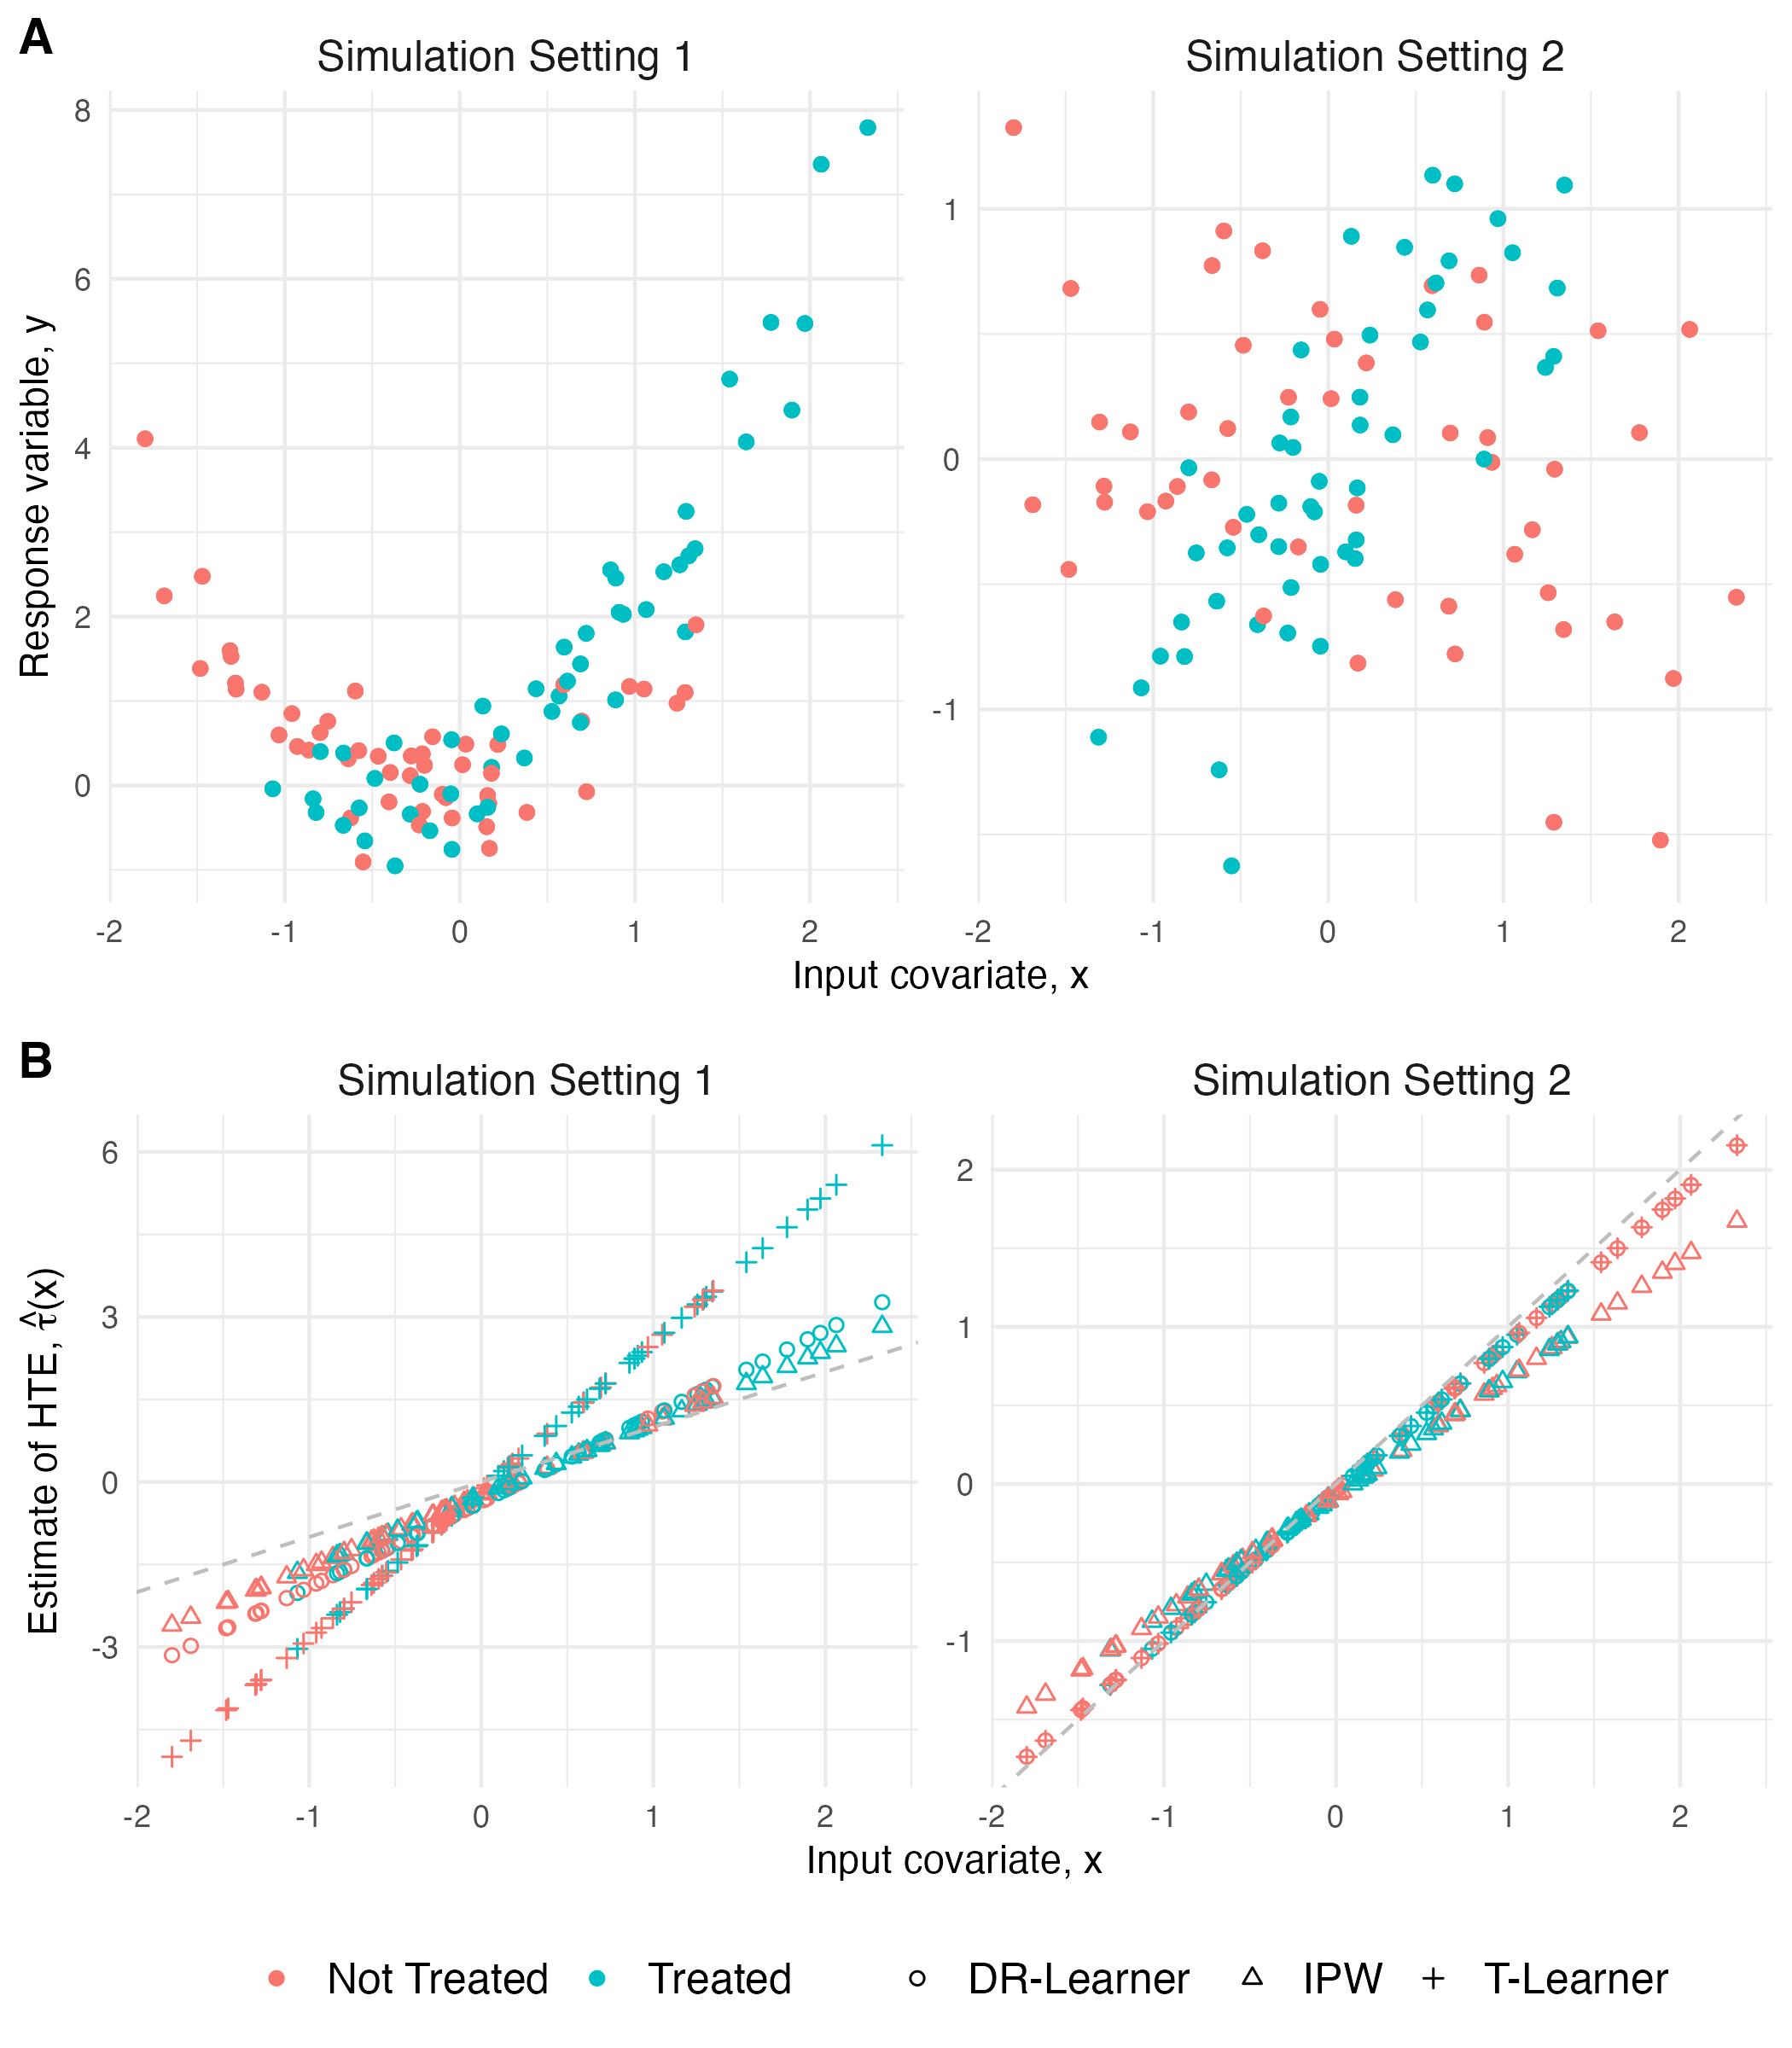
\includegraphics[width=\textwidth]{figures/chapter4/comp_figure_with_dr.png}
\caption{Simulation Settings~1~and~2 with \textbf{A}: the response variable $y$, and \textbf{B}: estimates of $\hat{\tau}(x)$ for each simulated data point according to the $T$-Learner (cross), \gls{ipw} (triangle), and DR-Learner (circle) strategies. The true \gls{cate}, $\tau(x)$, is shown with a grey dashed line.  \label{fig:comp_t_ipw_dr}}
\end{figure}

\subsection{Regularisation}
Another view of the two heuristic extremes described in Section~\ref{sec:doublerobustness} is as a balance between  `information sharing' across the estimated conditional regression functions $\muhat_0$ and $\muhat_1$, and allowing them to be as flexible as possible in order to capture nuances to the difference between them (i.e. the treatment effect). \citet{shalit_estimating_2017} proposed a method based on representation learning, in which three functions are learned: $\Phi(x), h_0(x), h_1(x)$, such that $\muhat_a(x) := h_a(\Phi(x))$. In this way information is shared between $\muhat_0$ and $\muhat_1$ via the embedding $\Phi$. The strength of this sharing is determining by applying a regularisation term to the loss function when fitting all three functions simultaneously, which penalises distributional divergence between $\Phi(X) \ | \ A = 1$ and $\Phi(X)  \ | \ A = 0$. 

\subsection{Causal forests}
\citep{athey_generalized_2019}

\section{Heterogeneous treatment effects applied to survival analysis}

\subsection{Forests again}

\subsection{Regularisation again}

\section{Application to a combined immunotherapy dataset}

\subsection{Validating TMB}

\subsection{Exploring more general markers}

\section{Conclusions}


\dobib % renders bibliography (only when compiling for chapter only)


\end{document}